\documentclass[12pt,letterpaper]{article}
\usepackage{graphicx,textcomp}
\usepackage{natbib}
\usepackage{setspace}
\usepackage{fullpage}
\usepackage{color}
\usepackage[reqno]{amsmath}
\usepackage{amsthm}
\usepackage{fancyvrb}
\usepackage{amssymb,enumerate}
\usepackage[all]{xy}
\usepackage{endnotes}
\usepackage{lscape}
\newtheorem{com}{Comment}
\usepackage{float}
\usepackage{hyperref}
\newtheorem{lem} {Lemma}
\newtheorem{prop}{Proposition}
\newtheorem{thm}{Theorem}
\newtheorem{defn}{Definition}
\newtheorem{cor}{Corollary}
\newtheorem{obs}{Observation}
\usepackage[compact]{titlesec}
\usepackage{dcolumn}
\usepackage{tikz}
\usetikzlibrary{arrows}
\usepackage{multirow}
\usepackage{xcolor}
\newcolumntype{.}{D{.}{.}{-1}}
\newcolumntype{d}[1]{D{.}{.}{#1}}
\definecolor{light-gray}{gray}{0.65}
\usepackage{url}
\usepackage{listings}
\usepackage{color}
\usepackage[T1]{fontenc}
\usepackage{booktabs}

\definecolor{codegreen}{rgb}{0,0.6,0}
\definecolor{codegray}{rgb}{0.5,0.5,0.5}
\definecolor{codepurple}{rgb}{0.58,0,0.82}
\definecolor{backcolour}{rgb}{0.95,0.95,0.92}

\lstdefinestyle{mystyle}{
	backgroundcolor=\color{backcolour},   
	commentstyle=\color{codegreen},
	keywordstyle=\color{magenta},
	numberstyle=\tiny\color{codegray},
	stringstyle=\color{codepurple},
	basicstyle=\footnotesize,
	breakatwhitespace=false,         
	breaklines=true,                 
	captionpos=b,                    
	keepspaces=true,                 
	numbers=left,                    
	numbersep=5pt,                  
	showspaces=false,                
	showstringspaces=false,
	showtabs=false,                  
	tabsize=2
}
\lstset{style=mystyle}
\newcommand{\Sref}[1]{Section~\ref{#1}}
\newtheorem{hyp}{Hypothesis}

\title{Problem Set 2}
\date{Due: October 15, 2023}
\author{Applied Stats/Quant Methods 1}

\begin{document}
	\maketitle
	\section*{Instructions}
\begin{itemize}
	\item Please show your work! You may lose points by simply writing in the answer. If the problem requires you to execute commands in \texttt{R}, please include the code you used to get your answers. Please also include the \texttt{.R} file that contains your code. If you are not sure if work needs to be shown for a particular problem, please ask.
	\item Your homework should be submitted electronically on GitHub.
	\item This problem set is due before 23:59 on Sunday October 15, 2023. No late assignments will be accepted.

\end{itemize}

	
	\vspace{.5cm}
	\section*{Question 1: Political Science}
		\vspace{.25cm}
	The following table was created using the data from a study run in a major Latin American city.\footnote{Fried, Lagunes, and Venkataramani (2010). ``Corruption and Inequality at the Crossroad: A Multimethod Study of Bribery and Discrimination in Latin America. \textit{Latin American Research Review}. 45 (1): 76-97.} As part of the experimental treatment in the study, one employee of the research team was chosen to make illegal left turns across traffic to draw the attention of the police officers on shift. Two employee drivers were upper class, two were lower class drivers, and the identity of the driver was randomly assigned per encounter. The researchers were interested in whether officers were more or less likely to solicit a bribe from drivers depending on their class (officers use phrases like, ``We can solve this the easy way'' to draw a bribe). The table below shows the resulting data.

\newpage
\begin{table}[h!]
	\centering
	\begin{tabular}{l | c c c }
		& Not Stopped & Bribe requested & Stopped/given warning \\
		\\[-1.8ex] 
		\hline \\[-1.8ex]
		Upper class & 14 & 6 & 7 \\
		Lower class & 7 & 7 & 1 \\
		\hline
	\end{tabular}
\end{table}

\begin{enumerate}
	
	\item [(a)]
	Calculate the $\chi^2$ test statistic by hand/manually (even better if you can do "by hand" in \texttt{R}).\\
	
	The $\chi^2$ test result is 3.791168. Below is the R code: 
	\lstinputlisting[language=R, firstline=8, lastline=35]{PS02_answers_Chenxi.R}
	\newpage
	\item [(b)]
	Now calculate the p-value from the test statistic you just created (in \texttt{R}).\footnote{Remember frequency should be $>$ 5 for all cells, but let's calculate the p-value here anyway.}  What do you conclude if $\alpha = 0.1$?\\
	
	Here is the null hypothesis and alternative hypothesis: \\
	H0:  These 2 variables in the population are not related and are independent of each others. \\
	H1: These 2 variables in the population are related to each others. \\
	Below is the R code: \\
	\lstinputlisting[language=R, firstline=37, lastline=60]{PS02_answers_Chenxi.R}
	p value = 0.1502306 > 0.1 = alpha; \\
	and $\chi^2_{0.1}$ = 3.791168 < 4.60517 = $\chi^2$(K=3) \\
	
	so we reject H1 and accept H0, we can think these 2 variables in the population are not related and are independent of each others.
	\newpage
	\item [(c)] Calculate the standardized residuals for each cell and put them in the table below.
	\vspace{1cm}
	
	\begin{table}[h]
		\centering
		\begin{tabular}{l | c c c }
			& Not Stopped & Bribe requested & Stopped/given warning \\
			\\[-1.8ex] 
			\hline \\[-1.8ex]
			Upper class  &0.14  &-0.82  &0.82  \\
			\\
			Lower class &-0.18  &1.09   &-1.10  \\

		\end{tabular}
	\end{table}
	Below is the R code:
	\lstinputlisting[language=R, firstline=62, lastline=74]{PS02_answers_Chenxi.R}
	\newpage
	\item [(d)] How might the standardized residuals help you interpret the results?  \\
	
	Firstly, we can determine whether the difference between the observed value and the expected value in each cell is significant.
	\begin{itemize}
		\item Since no cell has a standardized residual greater than 1.61, we can assume that there is no difference between the observed and expected values in these cells.
	\end{itemize}
	Secondly, we can judge the relationship of observed and expected value based on the positive and negative conditions of the residual. If we assume each standard residuals is significant, then we can conclude that: 
	\begin{itemize}
		\item For not stopped bribe categorical, upper class's observed value more than expected value; and lower class's observed value less than expected value.
		\item For bribe requested categorical, upper class's observed value less than expected value; and lower class's observed value more than expected value.
		\item For stopped or given warning categorical, upper class's observed value more than expected value, and lower class's observed value less than expected value.
	\end{itemize}
	
	Draw a heat map to visualize each cell's standard residual:
	\begin{figure}[h]
		\centering
		\caption{Heatmap: Standard Residual}
		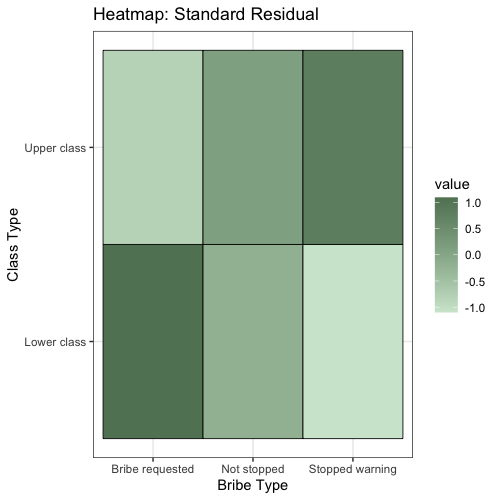
\includegraphics[scale=0.5]{Heatmap_Standard_Residual.png}
	\end{figure}
	\newpage
	Below is the R code:
	\lstinputlisting[language=R, firstline=76, lastline=95]{PS02_answers_Chenxi.R}
\end{enumerate}
\newpage

\section*{Question 2: Economics}
Chattopadhyay and Duflo were interested in whether women promote different policies than men.\footnote{Chattopadhyay and Duflo. (2004). ``Women as Policy Makers: Evidence from a Randomized Policy Experiment in India. \textit{Econometrica}. 72 (5), 1409-1443.} Answering this question with observational data is pretty difficult due to potential confounding problems (e.g. the districts that choose female politicians are likely to systematically differ in other aspects too). Hence, they exploit a randomized policy experiment in India, where since the mid-1990s, $\frac{1}{3}$ of village council heads have been randomly reserved for women. A subset of the data from West Bengal can be found at the following link: \url{https://raw.githubusercontent.com/kosukeimai/qss/master/PREDICTION/women.csv}\\

\noindent Each observation in the data set represents a village and there are two villages associated with one GP (i.e. a level of government is called "GP"). Figure~\ref{fig:women_desc} below shows the names and descriptions of the variables in the dataset. The authors hypothesize that female politicians are more likely to support policies female voters want. Researchers found that more women complain about the quality of drinking water than men. You need to estimate the effect of the reservation policy on the number of new or repaired drinking water facilities in the villages.
\vspace{.5cm}
\begin{figure}[h!]
	\caption{\footnotesize{Names and description of variables from Chattopadhyay and Duflo (2004).}}
	\vspace{.5cm}
	\centering
	\label{fig:women_desc}
	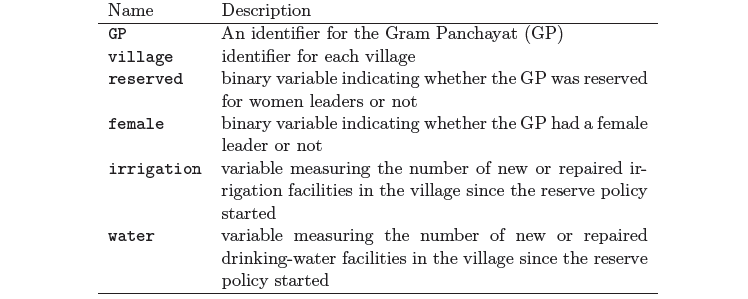
\includegraphics[width=1.1\textwidth]{women_desc.png}
\end{figure}		

\newpage
\begin{enumerate}
	\item [(a)] State a null and alternative (two-tailed) hypothesis. 
	\vspace{.5cm} \\
	$H_0$: Whether there are female leaders in a region \textbf{is not related to} with the number of newly built drinking water facilities in the region. \\
	
	$H_1$: Whether there are female leaders in a region \textbf{is related to} the number of newly built drinking water facilities in the region. \\
	
	And in math language, we can also make the statement like this: \\
	
	$H_0$: $\beta$ = 0\\
	$H_1$: $\beta$ $\neq$ 0 \\
	\vspace{.5cm} \\
	$\beta_0$ means the slop in regression model y = $\beta$x + $\alpha$ + $\varepsilon$
		
	\newpage
	\item [(b)] Run a bivariate regression to test this hypothesis in \texttt{R} (include your code!).
	\vspace{.5cm}\\
	Put "water" as dependent variable and binary variable "female" as independent variable. And because binary variable "female" is already a dummy variable, so we don't need to operate anything on it.\\
	
	Before we start regression model, we can draw a point plot to see the mean value of newly repaired drinking water facilities group by gender. \\
	\begin{figure}[h]
	\centering
	\caption{Point: Water Group by Gender}
	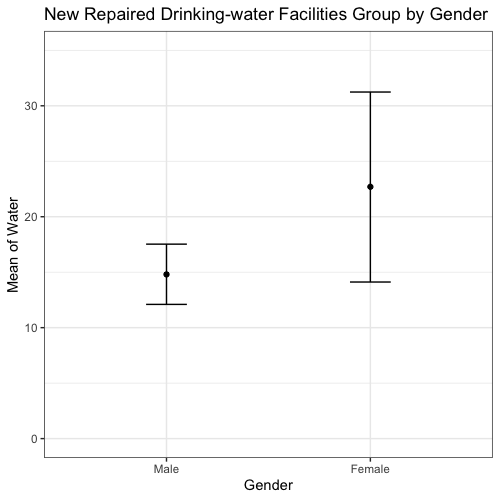
\includegraphics[scale=0.5]{Point&ci_Water_Groupby_Gender.png}
	\end{figure}
	
	Below is the R code of the plot:
	\lstinputlisting[language=R, firstline=101, lastline=130]{PS02_answers_Chenxi.R}
	
	Use R to get the data frame and create regression model: \\
	\lstinputlisting[language=R, firstline=132, lastline=134]{PS02_answers_Chenxi.R}
	
	And we can get the regression model table from R:
	
	\begin{table}[ht]
		\centering
		\caption{Abstract of Regression Model}
		\begin{tabular}{lcccc}
			\toprule
			& Estimate & Std. Error & t value & Pr($>|t|$) \\
			\midrule
			(Intercept) & 14.813 & 2.382 & 6.220 & 1.56e-09 *** \\
			female & 7.864 & 3.838 & 2.049 & 0.0413 * \\
			\bottomrule
		\end{tabular} 
	\end{table}
	Signif. codes:  0 ‘***’ 0.001 ‘**’ 0.01 ‘*’ 0.05 ‘.’ 0.1 ‘ ’ 1 \\
	
	Residual standard error: 33.51 on 320 degrees of freedom \\
	Multiple R-squared:  0.01295,	Adjusted R-squared:  0.009867 \\
	F-statistic: 4.199 on 1 and 320 DF,  p-value: 0.04126 \\
	
	Because the slop's p value is 0.0413 < 0.05, so it is significant.\\
	
	And this suggests we can reject $H_0$ and accept $H_1$, which means $\beta$ $\neq$ 0.

	
	\newpage
	\item [(c)] Interpret the coefficient estimate for reservation policy. \\
	
	According to (b), the regression model is: \\
	
	y = 7.864 x + 14.813 \\
	
	According the regression model, because we pass the F test and the slop is significant, so we can make this statement:\\
	
	In comparison to non-female leaders GP, the female leaders GP's newly repair drinking water facilities will expect to increase 7.864. \\
	
\end{enumerate}

\end{document}
